%%%%%%%%%%%%%%%%%%%%%%%%%%%%%%%%%%%%%%%%%%%%%%%%%%%
%% LaTeX book template                           %%
%% Author:  Amber Jain (http://amberj.devio.us/) %%
%% License: ISC license                          %%
%%%%%%%%%%%%%%%%%%%%%%%%%%%%%%%%%%%%%%%%%%%%%%%%%%%

\documentclass[a4paper,11pt]{book}
\usepackage[T1]{fontenc}
\usepackage[utf8]{inputenc}
\usepackage{lmodern}
\usepackage{subcaption}

%%%%%%%%%%%question block
\usepackage[tikz]{bclogo}
%%%%%%%%%%%%%%%%%%%%%%%%%%%%%%%%%%%%%%%%%%%%%%%%%%%%%%%%%
% Source: http://en.wikibooks.org/wiki/LaTeX/Hyperlinks %
%%%%%%%%%%%%%%%%%%%%%%%%%%%%%%%%%%%%%%%%%%%%%%%%%%%%%%%%%
\usepackage{hyperref}
\usepackage{graphicx}
\usepackage[english]{babel}
\usepackage{graphicx,amssymb,amstext,amsmath}
\usepackage{tikz}

\usepackage{mathtools}
\DeclarePairedDelimiter\ceil{\lceil}{\rceil}
\DeclarePairedDelimiter\floor{\lfloor}{\rfloor}
%%%%%%%%%%%%%%%%%%%%%%%%%%%%%%%%%%%%%%%%%%%%%%%%%%%%%%%%%%%%%%%%%%%%%%%%%%%%%%%%
% 'dedication' environment: To add a dedication paragraph at the start of book %
% Source: http://www.tug.org/pipermail/texhax/2010-June/015184.html            %
%%%%%%%%%%%%%%%%%%%%%%%%%%%%%%%%%%%%%%%%%%%%%%%%%%%%%%%%%%%%%%%%%%%%%%%%%%%%%%%%
\newenvironment{dedication}
{
   \cleardoublepage
   \thispagestyle{empty}
   \vspace*{\stretch{1}}
   \hfill\begin{minipage}[t]{0.66\textwidth}
   \raggedright
}
{
   \end{minipage}
   \vspace*{\stretch{3}}
   \clearpage
}
%%%%%%%%%%%%%%%%%%%%%%%%%%%%%%%%%%%%%%%%%%%%%%%%%%%%%%%%%%%%%%%%%%%%%%%%%%%%%%%%
% The setting for the exercise part: we can write the problems and the solutions at the same place, but can be displayed in the pdf at another place %
% Source: https://tex.stackexchange.com/questions/369265/math-book-how-to-write-exercise-and-answers %
%%%%%%%%%%%%%%%%%%%%%%%%%%%%%%%%%%%%%%%%%%%%%%%%%%%%%%%%%%%%%%%%%%%%%%%%%%%%%%%%
\usepackage{multicol}
\usepackage{multirow}
\usepackage{ifthen}
\newboolean{firstanswerofthechapter}  

\usepackage{xcolor}
\colorlet{lightcyan}{cyan!40!white}

\usepackage{chngcntr}
\usepackage{stackengine}

\usepackage{tasks}
%%%%%%%%%%%%%%%%%%%%%%%%%%%%%%%%%%%%%%%%%%%%%%%%%%%%%%%%%%%%%%%%%%%%%%%%%%%%%%%%
% The setting for the chapter style %
% Source: https://texblog.org/2012/07/03/fancy-latex-chapter-styles/ %
%%%%%%%%%%%%%%%%%%%%%%%%%%%%%%%%%%%%%%%%%%%%%%%%%%%%%%%%%%%%%%%%%%%%%%%%%%%%%%%%

\usepackage[Sonny]{fncychap}
% \usepackage{titlesec}
 
% \titleformat
% {\chapter} % command
% [display] % shape
% {\bfseries\Large}%\itshape} % format
% {Chapter No. \ \thechapter} % label
% {0.5ex} % sep
% {
%     \rule{\textwidth}{1pt}
%     \vspace{1ex}
%     \centering
% } % before-code
% [
% \vspace{-0.5ex}%
% \rule{\textwidth}{0.3pt}
% ] % after-code
%%%%%%%%%%%%%%%%%%%%%%%%%%%%%%%%%%%%%%%%%%%%%%%%%%%%%%%%%%%%%%%%%%%%%%%%%%%%%%%%
% The setting for the examples style %
% Source: https://tex.stackexchange.com/questions/295589/how-to-enumerate-a-problem-set-in-a-book-accordingly-with-the-chapter-number %
%%%%%%%%%%%%%%%%%%%%%%%%%%%%%%%%%%%%%%%%%%%%%%%%%%%%%%%%%%%%%%%%%%%%%%%%%%%%%%%%
\usepackage{enumitem}
\newlist{examples}{enumerate}{1}
\setlist[examples]{label={\thechapter.\arabic*}}

% \BeforeBeginEnvironment{example}{\vspace{\baselineskip}}
% \AfterEndEnvironment{example}{\vspace{\baselineskip}}
% \BeforeBeginEnvironment{sourcecode}{\vspace{\baselineskip}}
% \AfterEndEnvironment{sourcecode}{\vspace{\baselineskip}}

\newlength{\longestlabel}
\settowidth{\longestlabel}{\bfseries viii.}
\settasks{counter-format={tsk[r].}, label-format={\bfseries}, label-width=\longestlabel,
    item-indent=0pt, label-offset=2pt, column-sep={10pt}}

\usepackage[lastexercise,answerdelayed]{exercise}
\counterwithin{Exercise}{chapter}
\counterwithin{Answer}{chapter}
\renewcounter{Exercise}[chapter]
\newcommand{\QuestionNB}{\bfseries\arabic{Question}.\ }
\renewcommand{\ExerciseName}{EXERCISES}
\renewcommand{\ExerciseHeader}{\noindent\def\stackalignment{l}% code from https://tex.stackexchange.com/a/195118/101651
    \stackunder[0pt]{\colorbox{cyan}{\textcolor{white}{\textbf{\LARGE\ExerciseHeaderNB\;\large\ExerciseName}}}}{\textcolor{lightcyan}{\rule{\linewidth}{2pt}}}\medskip}
\renewcommand{\AnswerName}{Exercises}
\renewcommand{\AnswerHeader}{\ifthenelse{\boolean{firstanswerofthechapter}}%
    {\bigskip\noindent\textcolor{cyan}{\textbf{CHAPTER \thechapter}}\newline\newline%
        \noindent\bfseries\emph{\textcolor{cyan}{\AnswerName\ \ExerciseHeaderNB, page %
                \pageref{\AnswerRef}}}\smallskip}
    {\noindent\bfseries\emph{\textcolor{cyan}{\AnswerName\ \ExerciseHeaderNB, page \pageref{\AnswerRef}}}\smallskip}}
\setlength{\QuestionIndent}{16pt}


%%%%%%%%%%%%%%%%%%%%%%%%%%%%%%%%%%%%%%%%%%%%%%%%%%%%%%%%%%%%%%%%%%%%%%%
% design the code listing
%%%%%%%%%%%%%%%%%%%%%%%%%%%%%%%%%%%%%%%%%%%%%%%%%%%%%%%%%%%%%%%%%%%%%%%
\usepackage{listings}

       
\usepackage{color}
 
\definecolor{codegreen}{rgb}{0,0.6,0}
\definecolor{codegray}{rgb}{0.5,0.5,0.5}
\definecolor{codepurple}{rgb}{0.58,0,0.82}
\definecolor{backcolour}{rgb}{0.95,0.95,0.92}
 
\lstdefinestyle{mystyle}{
    backgroundcolor=\color{backcolour},   
    commentstyle=\color{codegreen},
    keywordstyle=\color{magenta},
    numberstyle=\tiny\color{codegray},
    stringstyle=\color{codepurple},
    basicstyle=\footnotesize,
    breakatwhitespace=false,         
    breaklines=true,                 
    captionpos=b,                    
    keepspaces=true,                 
    numbers=left,                    
    numbersep=5pt,                  
    showspaces=false,                
    showstringspaces=false,
    showtabs=false,                  
    tabsize=2
}
 
\lstset{style=mystyle}
%%%%%%%%%%%%%%%%%%%%%%%%%%%%%%%%%%%%%%%%%%%%%%%%%%%%%%%%%%%%%%%%%%%%%%%%%%%%%%%
% package enumberate with different style                                     %
%%%%%%%%%%%%%%%%%%%%%%%%%%%%%%%%%%%%%%%%%%%%%%%%%%%%%%%%%%%%%%%%%%%%%%%%%%%%%%%
\usepackage{enumitem} %[label=(\alph*)], [label=(\Alph*)], [label=(\roman*)]
\usepackage{titlesec}

\setcounter{secnumdepth}{3} %subsubsection and paragraph

\newlist{inparaenum}{enumerate}{2}% allow two levels of nesting in an enumerate-like environment
\setlist[inparaenum]{nosep}% compact spacing for all nesting levels
\setlist[inparaenum,1]{label=\bfseries\arabic*.}% labels for top level
\setlist[inparaenum,2]{label=\arabic{inparaenumi}\emph{\alph*})}% labels for second level

%%%%%%%%%%%%%%%%%%%%%%%%%%%%%%%%%%%%%%%%%%%%%%%%%%%%%%%%%%%%%%%%%%%%%%%%%%%%%%%%%
% better align the equation                                                     %
%%%%%%%%%%%%%%%%%%%%%%%%%%%%%%%%%%%%%%%%%%%%%%%%%%%%%%%%%%%%%%%%%%%%%%%%%%%%%%%%%%
\usepackage{amsmath}
\usepackage{subfiles}
\usepackage{subcaption} 
% \usepackage{blindtext}



%%%%%%%%%%%%%%%%%%%%%%%%%%%%%%%%%%%%%%%%%%%%%%%%
% Chapter quote at the start of chapter        %
% Source: http://tex.stackexchange.com/a/53380 %
%%%%%%%%%%%%%%%%%%%%%%%%%%%%%%%%%%%%%%%%%%%%%%%%
\makeatletter
\renewcommand{\@chapapp}{}% Not necessary...
\newenvironment{chapquote}[2][2em]
  {\setlength{\@tempdima}{#1}%
   \def\chapquote@author{#2}%
   \parshape 1 \@tempdima \dimexpr\textwidth-2\@tempdima\relax%
   \itshape}
  {\par\normalfont\hfill--\ \chapquote@author\hspace*{\@tempdima}\par\bigskip}
\makeatother

\title{\Huge \textbf{Non-linear Recursive Backtracking}   }

% \title{\Huge \textbf{The Comprehensive Coding Interview Guide}  \footnote{This is a footnote.} \\ \huge  Cracking LeetCode Problems Using Python \footnote{This is yet another footnote.}}

% \title{\Huge \textbf{Notebook of Data Structures and Algorithms  for Coding Interview }  \footnote{This is a footnote.} \\ \huge  Cracking LeetCode Problems Using Python \footnote{This is yet another footnote.}}
% Author
\author{\textsc{Li Yin}\thanks{\url{www.liyinscience.com}}}
\begin{document}
\frontmatter
\maketitle

% \chapter{Linear Search}
% \label{chapter_linear_searching}
% \subfile{chapters/part3/searching}
% \section{Binary Search}
% \label{sec_binary_search}
% \subfile{chapters/part3/search/binary_search}

% \chapter{Heap and Priority Queue}
% \label{chapter_heap_priority_queue}
% \subfile{chapters/part2/heap_priority_queue}

% \chapter{Bit Manipulation}
% \subfile{chapters/chapter_15_bit-manipulation }
% \label{tree_problem}
\chapter{Purged Recurrence relation}
\section{Solve Recurrence Function}


\subsection{Iteration and Recursion Tree} 
\subsection{Characteristic Root Technique}
In this section, we use the overlapping subproblem related complexity function to show how we use recursion tree and characteristic root technique to get the same time complexity. 
\begin{align}
\label{complexity_eq_fibonacci_1}
    T(n)&=T(n-1)+T(n-2)+O(1)\\
    &=(T(n-2)+T(n-3)+O(1))+(T(n-3)+T(n-4)+O(1))+O(1)\notag\\
    &=...
\end{align}
It is actually very difficult for us to keep expanding, because the item of T(k) will double each time we try to expand it, this is eventually grow exponentially. If we insist on expanding, we can use recursion tree method. We can get a tighter bound using recursion tree method, where instead we just use $L_k$ to represent each level and we can do simple merge of different term, which is easier for us to find rules: 
\begin{align}
\label{complexity_eq_fibonacci_1}
    T(n)&=T(n-1)+T(n-2)         +          O(1)\\
    L_1&=\cancel{T(n-1)+T(n-2)}         +          O(1)\\
    L_2&=\cancel{(T(n-2)+2T(n-3)+T(n-4))}+O(2^1)\notag\\
    L_3&=\cancel{(T(n-3)+3T(n-4)+3T(n-5)+T(n-6))}+O(2^2)\notag\\
    L_4&=\cancel{(T(n-4)+4T(n-5)+6T(n-6)+4T(n-7)+T(n-8))}+O(2^3)\notag\\
    L_k&=\underbrace{(T(n-k)+...+T(n-k-k))}_\text{T(c) Reminder}+\underbrace{O(2^{k-1})}_\text{Summation of f(n) at each level}\notag
\end{align}
The last level we will have $T(n-2k)=T(1)=1$, which states $k=n/2$. For the final time complexity, it will be composed of two parts: (1) the summation of the $f(n)$ part over different level, which is $\sum_{i=0}^{k-1} 2^i$; and (2) the reminder of the $T(c)$, which states the cost for trivial case. It is $(T(n-n/2)+...+T(1))$, and according to the rule of the coefficient, $(T(n-n/2)+...+T(1))>=2^k$. With the math formula that $t^0+t^1+...+t^n=\frac{1-t^{n+1}}{1-t}$. Therefore, we can rewrite our time complexity function as:
\begin{align}
    T(n)&\geq \sum_{i=0}^{k-1} 2^i + 2^k\\
    &=\sum_{i=0}^{k} 2^k \\
    &=\frac{1-2^{k+1}}{1-2} \\
    &=2^{k+1}\\
    &=2^{n/2}
\end{align}

It would be reasonable for us to guess $r^n$. For this type of recursion, it is hard to find the tight bound, we can do the following simplification to find a lower bound instead, and replace each term with out guess
\begin{align}
\label{complexity_eq_fibonacci_2}
    T(n)&\geq T(n-1)+T(n-2)\\
    r^n &\geq r^{(n-1)}+r^{(n-2)}\notag\\
    r^{(n-2)}(r^2-r-1)&\geq 0
\end{align}
With some math knowledge that given a general quadratic formula as $ax^2+bx+c=0$, the solution will be $x=\frac{-b\pm\sqrt{b^2-4ac}}{2a}$. With the formula, we get the solution for equation $(r^2-r-1)=0$, which is $r=\frac{1\pm\sqrt{5}}{2}$:
\begin{align}
\label{complexity_eq_fibonacci_3}
    T(n)&\geq A(\frac{1+\sqrt{5}}{2})^n+B(\frac{1-\sqrt{5}}{2})^n\\
    T(n)&\geq A(\frac{1+\sqrt{5}}{2})^n\\
    T(n)&\geq2^{n/2}\\
    T(n) &= \Omega(2^{n/2})
\end{align}
\subsection{Master Method} Recursion tree and the master theorem are the main ways we rely on to answer the time complexity for a divide and conquer method of form shown in Eq.~\ref{bt_time_1}. The master method is probably the easiest way to come up with the computational complexity analysis. It is a theorem that are proved by researchers, and we just need to learn how to use them. The master theorem goes:
\begin{align}
\label{bt_time_1}
    T(n)=aT(n/b)+f(n)
\end{align}

For Eq.~\ref{bt_time_1}, let $a\geq1, b>1$, and $f(n)$ is asymptotically positive function. This represents that using divide and conquer, we divide a problem of size $n$ into $a$ subproblems and each of size $n/b$. The $a$ subproblems are solved recursively, each in time $T(n/b)$. Plus with the cost of $f(n)$, which represents the cost of dividing the problem and combining results of the subprolems, we get the time complexity of size $n$. 

The master theorem states that for Eq.~\ref{bt_time_1}, $T(n)$ has three following asymptotic bounds.  
\begin{enumerate}
    \item If $f(n) = O(n^{\log_b a - \epsilon})$ for constant $\epsilon>0$, then we get $T(n) = \Theta(n^{\log_b a})$.
    \item If $f(n) = \Theta(n^{\log_b a })$, then we get $T(n) = \Theta(n^{\log_b a} \log n)$.
    \item If $f(n) = \Omega(n^{\log_b a + \epsilon})$ for constant $\epsilon>0$, and if $a f(n/b)\leq cf(n)$ for constant $c<1$ and all sufficiently large $n$, then we get $T(n) = \Theta(f(n))$.
\end{enumerate}

\paragraph{Apply Master Method} To apply master method given a function $T(n)$, we first compute $n^{\log_b a}$, and then compare $f(n)$ with $n^{\log_b a}$. Intuitively, the larger of the two functions determines the solution to the recurrence. As shown in the following equation of case 1 and 3. For case 2, these two functions are of the same size, we multiply it by a logarithmic factor. 
\begin{align}
    f(n) &> n^{\log_b a}, \text{case 3}, T(n)= \Theta(f(n))\\
    f(n) &< n^{\log_b a}, \text{case 1}, T(n)=\Theta(n^{\log_b a})\\
f(n) &= n^{\log_b a}, a f(n/b)\leq cf(n), \text{case 2}, T(n)=\Theta(n^{\log_b a} \log n)
\end{align}
Note that the comparison will be polynomial comparison. 

\paragraph{When We cant Use Master Method} The three cases do not cover all the possibilities for $f(n)$. There is a gap between case 1 and 2 when $f(n)$ is smaller but not polynomially smaller. Similarly, there is a gap between case 3 and 2 when $f(n)$ is larger but not polynomially larger. Or if the regularity condition in case 3 fails to hold, we can not use master method. We go back to other techniques instead. 




% \paragraph{Solving  Non-overlapping Recurrence Function:}



% \subsubsection{Recursion Tree Method}
% Drawing out a recursion tree serves as a straightforward way to come up with a good guess. Normally we can tolerate a small amount of "sloppiness", because later on, we can prove the complexity with substitution method discussed in the last section. However, when we are drawing the recursion tree, if we are careful enough and summing up the costs from each level and each node, we can use is as a direct proof of the solution to the recurrence. 

% In the corresponding recursion tree for recurrence equation in divide and conquer, each node represents the cost of a single subproblem somewhere in the set of recursive function invocations. We sum the costs within each level of the tree to obtain a set of per-level costs, and then we sum all the per-level costs to determine the total cost of all levels of the recursion. Let's look at one example for given recursion $T(n) = 3T(\floor*{n/4}) + \Theta(n^2)$. We replace $\Theta(n^2) = cn^2$, where $c>0$. $cn^2$ is the cost we pay to divide a problem with $n$ input size to three problems each with $n/4$ input size and combine the solution of the subproblems to solve the current problem.  We first expand $T(n)$, and put the cost $cn^2$ at the root, and with three children each noted with $T(n/4)$. Then we recursively replace $T(n/4)$ with the cost and its subproblem till the size of each subproblem to be 1, which means we get to the leaves. The computational complexity for this recursion would be the sum of all layers's costs. And we assume $T(1)=1$.
% \begin{figure}[h]
%     \centering
%     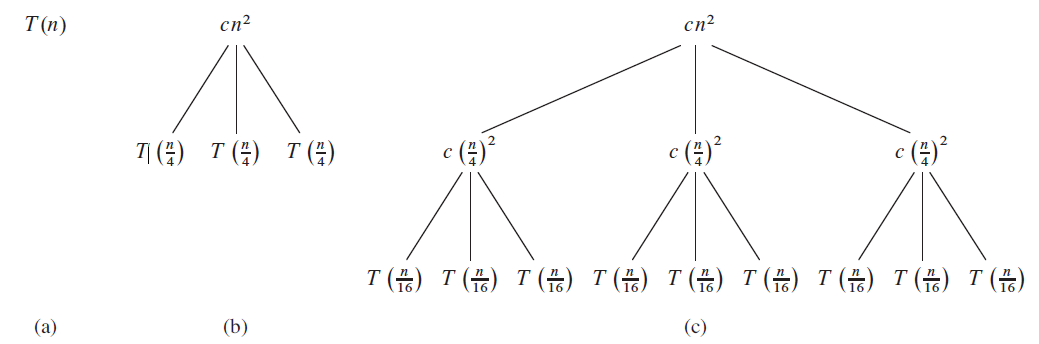
\includegraphics[width=0.8\columnwidth]{fig/recursive_tree_1.png}
%     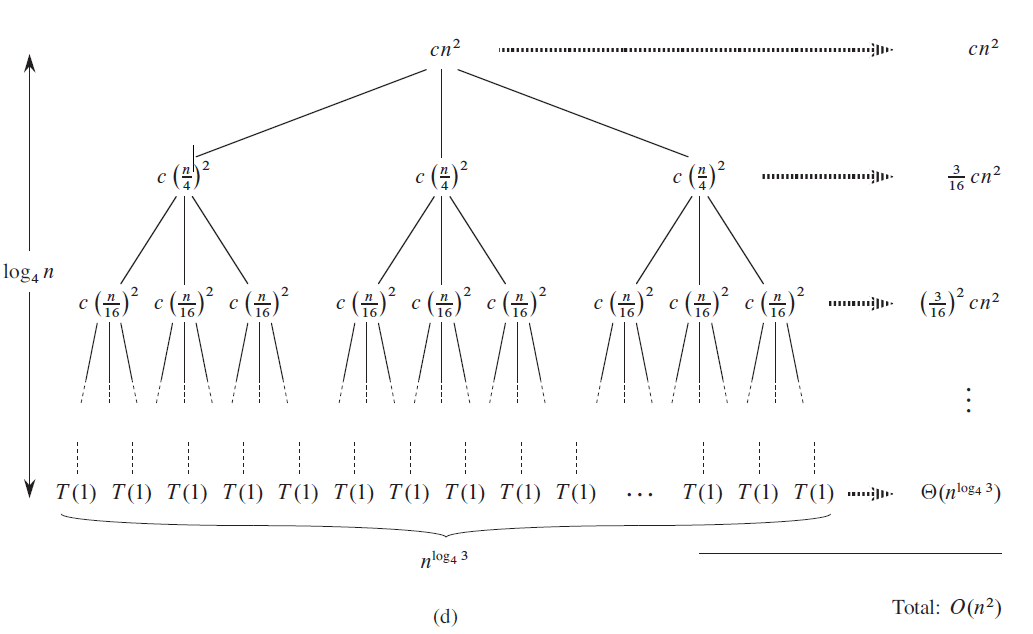
\includegraphics[width=0.8\columnwidth]{fig/recursive_tree_2.png}
%     \caption{The process to construct a recursive tree for $T(n) = 3T(\floor*{n/4}) + cn^2$}
%     \label{fig:recursive_tree}
% \end{figure}
% \begin{equation} \label{eg_recurrence_5}
% \begin{split}
% T(n) & = cn^2+\frac{3}{16}cn^2+(\frac{3}{16})^2cn^2+...+(\frac{3}{16})^{\log_4 {n-1}}cn^2+\Theta(n^{\log_4 3})\\
% & = \sum_{i=0}^{\log_4 {n-1}}(\frac{3}{16})^{i}cn^2+\Theta(n^{\log_4 3})\\
% &< \sum_{i=0}^{\infty}(\frac{3}{16})^{i}cn^2+\Theta(n^{\log_4 3})\\
% & = \frac{1}{1-(3/16)} cn^2+\Theta(n^{\log_4 3})\\
% & = O(n^2).
% \end{split}
% \end{equation}
% \subsubsection{Master Method}

\end{document}